%%%%%%%%%%%%%%%%%%%%%%%%%%%%%%%%%%%%%%%%%
% Journal Article
% LaTeX Template
% Version 1.4 (15/5/16)
%
% This template has been downloaded from:
% http://www.LaTeXTemplates.com
%
% Original author:
% Frits Wenneker (http://www.howtotex.com) with extensive modifications by
% Vel (vel@LaTeXTemplates.com)
%
% License:
% CC BY-NC-SA 3.0 (http://creativecommons.org/licenses/by-nc-sa/3.0/)
%
%%%%%%%%%%%%%%%%%%%%%%%%%%%%%%%%%%%%%%%%%
%MODIFICACIÓN-MARCELO OYANEDER LABARCA- AJUSTE A INFORME DIQ, USACH%%%%%
%----------------------------------------------------------------------------------------
%	PACKAGES AND OTHER DOCUMENT CONFIGURATIONS
%----------------------------------------------------------------------------------------

\documentclass[twoside,twocolumn,letter,10pt]{article}

\usepackage{blindtext} % Package to generate dummy text throughout this template 
\usepackage{graphicx} %Package to insert images and graphics
\usepackage{amsmath}
\newcommand*{\Scale}[2][4]{\scalebox{#1}{$#2$}}%

\usepackage{xcolor} %font color tables
\usepackage{colortbl} %fill color tables

\usepackage[T1]{fontenc}%fuente
%\usepackage[condensed,sfdefault]{universalis}%fuente 
%\usepackage[scaled]{helvet} %fuente helvetica
%\usepackage[scaled]{uarial} %fuente uarial
\usepackage{fontspec} % ESTA LINEA COMPILAR CON XELATEX
\setmainfont{Arial} %ESTA LINEA COMPILAR CON XELATEX
\renewcommand*\familydefault{\sfdefault}%fuente
\linespread{1.5} % Line spacing 

\usepackage[spanish]{babel} % Language hyphenation and typographical rules

\usepackage[left=3cm,top=2.5cm,right=3cm,bottom=2.5cm]{geometry} %margenes
\usepackage[hang, small,labelfont=bf,up,textfont=it,up]{caption} % Custom captions under/above floats in tables or figures
\usepackage{booktabs} % Horizontal rules in tables

\usepackage{lettrine} % The lettrine is the first enlarged letter at the beginning of the text

\usepackage{enumitem} % Customized lists
\setlist[itemize]{noitemsep} % Make itemize lists more compact

\usepackage{abstract} % Allows abstract customization
\renewcommand{\abstractnamefont}{\normalfont\bfseries} % Set the "Abstract" text to bold
\renewcommand{\abstracttextfont}{\normalfont\small\itshape} % Set the abstract itself to small italic text

\usepackage{titlesec} % Allows customization of titles
\renewcommand\thesection{\Roman{section}} % Roman numerals for the sections
\renewcommand\thesubsection{\roman{subsection}} % roman numerals for subsections
\titleformat{\section}[block]{\large\scshape\centering}{\thesection.}{1em}{} % Change the look of the section titles
\titleformat{\subsection}[block]{\large}{\thesubsection.}{1em}{} % Change the look of the section titles

\usepackage{fancyhdr} % Headers and footers
\pagestyle{fancy} % All pages have headers and footers
\fancyhead{} % Blank out the default header
\fancyfoot{} % Blank out the default footer
\fancyhead[C]{Intercambiador de calor $\bullet$ Junio 2019 $\bullet$ Laboratorio transferencia de calor Ingeniería civil Química I-2019} % Custom header text
\fancyfoot[RO,RE]{\thepage} % Custom footer text

\usepackage{titling} % Customizing the title section

\usepackage{hyperref} % For hyperlinks in the PDF

%----------------------------------------------------------------------------------------
%	TITLE SECTION
%----------------------------------------------------------------------------------------

\setlength{\droptitle}{-4\baselineskip} % Move the title up

\pretitle{\begin{center}\Huge\bfseries} % Article title formatting
\posttitle{\end{center}} % Article title closing formatting
\title{Intercambiador de calor } % Article title
\author{%
\textsc{A\lowercase{ntara Guajardo}}\thanks{Profesora laboratorio} \\[0.2ex] % Your name
\normalsize Universidad de Santiago de Chile \\ % Your institution
\normalsize \href{mailto:antara.guajardo@usach.cl}{antara.guajardo@usach.cl} % Your email address
\and % Uncomment if 2 authors are required, duplicate these 4 lines if more
\textsc{Dayana Lucero}\thanks{Ayudante laboratorio} \\[0.2ex] % Second author's name
\normalsize Universidad de Santiago de Chile \\ % Second author's institution
\normalsize \href{mailto:dayana.lucero@usach.cl}{dayana.lucero@usach.cl} % Second author's email address
\and % Uncomment if 2 authors are required, duplicate these 4 lines if more
\textsc{Marcelo Oyaneder}\thanks{Ayudante laboratorio} \\[0.2ex] % Second author's name
\normalsize Universidad de Santiago de Chile \\ % Second author's institution
\normalsize \href{mailto:marcelo.oyaneder@usach.cl}{marcelo.oyaneder@usach.cl} % Second author's email address
}
\date{} % Leave empty to omit a date
\renewcommand{\maketitlehookd}{%
\begin{abstract}
\noindent  Un intercambiador de calor es un aparato que facilita el intercambio de calor entre dos fluidos que se encuentran a temperaturas diferentes y evitan al mismo tiempo que se mezclen entre sí. El intercambiador de calor a analizar en esta experiencia recibe el nombre de tubos y coraza y se caracteriza por contener en él un gran número de tubos, empacados en un casco con sus ejes paralelos al de éste. La transferencia de calor tiene lugar a medida que uno de los fluidos se mueve por dentro de los tubos, en tanto que el otro se mueve por fuera de éstos, pasando por la coraza. \cite{cengel2014heat}
\end{abstract}
}

%----------------------------------------------------------------------------------------

\begin{document}

% Print the title
\maketitle

%----------------------------------------------------------------------------------------
%	ARTICLE CONTENTS
%----------------------------------------------------------------------------------------

\section{Introducción}

\indent Se realizará el análisis de un intercambiador de calor del tipo 1:2, como el mostrado a continuación.

\begin{figure}[hbtp]
\caption{Intercambiador de tubos y carcasa 1:2, extraído de \cite{cengel2014heat} }
\centering
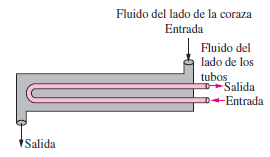
\includegraphics[scale=0.75]{imagenes/shellandtubes.png}
\end{figure}

En este al igual que en el presente en el laboratorio de operaciones unitarias (LOPU), se encontrarán dos entradas y salidas. En las entradas se encuentra una para el líquido frío, el cual circulará dentro de los tubos y otra para el fluido caliente, en este caso vapor saturado proveniente desde la caldera, el cual circulará por el interior de la carcasa. Respecto a las salidas se encuentra una para el líquido frío el cual absorbe calor desde el fluido caliente y la restante es para el fluido caliente, pero en este caso sale a una temperatura menor a la de entrada.



%------------------------------------------------
\newpage
\section{Procedimiento experimental}
\subsection{Calibración placa orificio}
\begin{figure}[hbtp]
\caption{Diagrama de flujo correspondiente a la calibración de la placa orificio}
\centering
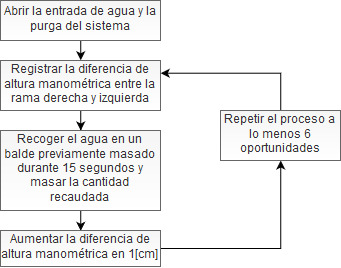
\includegraphics[scale=0.5]{imagenes/placaorificio.jpg}
\end{figure}

\newpage
\subsection{Operación del intercambiador de calor}
\begin{figure}[hbtp]
\caption{Diagrama de flujo correspondiente a la operación del intercambiador de calor}
\centering
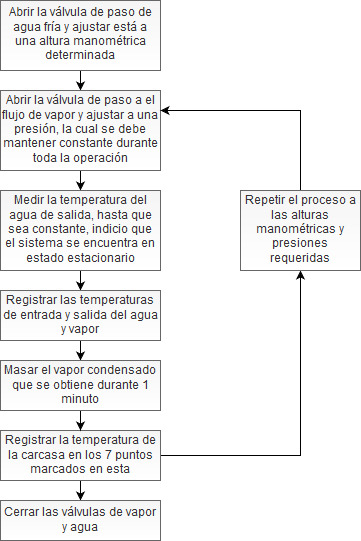
\includegraphics[scale=0.5]{imagenes/heatexchanger.jpg}
\end{figure}


%------------------------------------------------
\newpage
\section{Objetivos}
\begin{itemize}
\item{Objetivo general:}
\begin{itemize}
\item{Analizar el proceso de transferencia de calor en un intercambiador de tubo y coraza con vapor de agua como fluido calefactor, para la condición de caudal o presión constante}
\end{itemize}
\item{Objetivos específicos:}
\begin{itemize}
\item{Determinar los flujos de energía involucrados en el sistema}
\item{Calcular la eficiencia del intercambiador de calor}
\item{Determinar la resistencia a la incrustación del sistema}
\end{itemize}
\end{itemize}

%------------------------------------------------
\newpage
\section{Datos de diseño}
\begin{itemize}
\item{Datos del intercambiador utilizado en la experiencia.}

% Table generated by Excel2LaTeX from sheet 'Hoja1'
\begin{table}[htbp]
  \centering
  \caption{Datos del intercambiador utilizado en la experiencia.}
    \begin{tabular}{p{5.355em}c}
    \toprule
    \multicolumn{2}{p{10.71em}}{Intercambiador de tubos y carcasa 1:2} \\
    \midrule
    \midrule
    Número de pasos & 2 \\
    Número de filas & 4 \\
    \end{tabular}%
  \label{tab:addlabel}%
\end{table}%

\item{Dimensiones del intercambiador utilizado en la experiencia.}
% Table generated by Excel2LaTeX from sheet 'Hoja1'
\begin{table}[htbp]
  \centering
  \caption{Dimensiones del intercambiador utilizado en la experiencia.}
    \begin{tabular}{lc}
    \toprule
    \multicolumn{1}{c}{Dimensión} & \multicolumn{1}{p{5.355em}}{Valor [m]} \\
    \midrule
    \midrule
    $D_{i,t}$     & 0,01 \\
    $D_{o,t}$     & 0,013 \\
    $D_{i,c}$     & 0,107 \\
    $D_{o,c}$     & 0,115 \\
    $L_c$     & 0,8 \\
    $L_t$     & 0,825 \\
    $N_t$     & 7\footnote{Recordar que son dos etapas, por lo tanto, en el interior hay 14 tubos.} \\
    \end{tabular}%
  \label{tab:addlabel}%
\end{table}%


\end{itemize}

%------------------------------------------------
\newpage
\section{Correlaciones}
\begin{itemize}
\item{Chuchill \& Chu: Se utiliza para obtener el coeficiente de transferencia de calor convectivo para el aíre \cite{churchill1975correlating}. }
\[\Scale[0.92]{$$Nu^{1/2}=0,60+0,387\cdot\left(\frac{Gr \cdot Pr}{[1+(0,559/Pr)^{9/16}]^{16/9}}\right)^{1/6}$$}\]
\item{Chen: Se utiliza para obtener el coeficiente de transferencia de calor para el vapor \cite{chen1966correlation}. }
\[\Scale[1]{$$\overline{h_{steam}}=0,725\cdot \left(\frac{g\cdot\rho_l \cdot(\rho_l -\rho_v)\cdot\Delta h\cdot k_l^3}{\mu_l \cdot(T_{sat}-T_{wall})\cdot D\cdot N}\right)^{1/4}$$}\]
\item{Dittus \& Boelter: Se utiliza para obtener el coeficiente de transferencia de calor convectivo para el flujo agua \cite{heiss1951nomograph}.}
$$Nu=0,023\cdot Re^{0,8}\cdot Pr^{0,4}$$
\end{itemize}


%------------------------------------------------
\newpage
\section{Cálculos}
\begin{itemize}
%--------------------------------------------------------------------------------------
\item{Procedimiento:}
\begin{itemize}
\item{A través de la presión manometrica es posible obtener la temperatura de saturación. La cual permite obtener las siguientes propiedades físicas $\Delta h$ y $\overline{C_{p,steam}}$. Con estos valores es posible obtener el calor cedido $(Q_{ced})$}
\item{A través de la temperatura media del líquido $\overline{T_{water}}$ es posible obtener $\overline{C_{p,water}}$, lo que posteriormente permitirá obtener el calor absorbido $(Q_{abs})$ }
\item{A través de $\overline{T_{shell}}$ y $T_{\infty}$, es posible obtener una temperatura de film $(T_{film})$. Con este valor calcular los parámetros necesarios para la utilización de la correlación de \textit{Churchill \& Chu} que permitirá obtener el calor de aíre $(Q_{air})$, es importante considerar que el área de transferencia de calor en este caso corresponde a la carcasa. }
\item{Todos los pasos anteriores nos permiten obtener una diferencia entre el calor perdido a través de un balance de energía y por correlación. }
\newpage
\item{Para la obtención del calor de vapor $(Q_{steam})$ y calor de agua $(Q_{water})$ se deberá hacer una iteración a la temperatura de pared $(T_{wall})$, ya que en ambos casos está se ve involucrada para el calculo de la temperatura de film del vapor $(T_{film,steam})$ como la del agua $(T_{film,water})$. Con cada una de estas se calculará las propiedades físicas necesarias para la utilización de la correlación de \textit{Chen } y \textit{Dittus \& Boelter}. Lo que permitirá obtener la temperatura de pared y con esto la entalpia de vapor $(\overline{h_{steam}})$ y la entalpia del líquido $(\overline{h_{water}})$. }
\item{Con los valores anteriores es posible obtener el coeficiente de transferencia de calor limpio $(U_C)$, el cual es posible calcular mediante la siguiente ecuación.
$$\frac{1}{U_c}=\frac{1}{\overline{h_{water}}}+\frac{1}{\overline{h_{steam}}}$$}
\item{Para calcular el factor de incrustración $(R_D)$ presente en el sistema, primero es necesario calcular el coeficiente de transferencia de calor sucio $(U_D)$, que se puede calcular mediante la siguiente ecuación.
$$\frac{1}{U_D}=\frac{N_t \cdot A_{i,tube} \cdot \Delta T_{mL} \cdot F}{Q_{water}}$$
Calculado este ultimo, la obtención de $R_D$ se hace mediante su definición.
$$R_D=\frac{1}{U_D}+\frac{1}{U_C}$$}
\end{itemize}
%---------------------------------------------------------------------------------
\newpage
\item{Cuestionario, \textbf{las preguntas presentes acá no las debe responder en su informe, pero son vitales para obtener los resultados de este}:}
\begin{itemize}
\item{¿Las temperaturas de film $T_{film,steam}$ y $T_{film,water}$ se pueden considerar como una sola?}
\item{¿Es posible considerar iguales el área externa como interna de la tubería?}
\item{¿Para el balance de energía total, es posible despreciar las perdidas de calor por el aíre $(Q_{air})$?} 
\item{Respecto al $Q_{ced}$, ¿se debe considerar la propiedad $\overline{C_{p,steam}}$ para el calculo de este?, y si no, ¿en qué ocasiones se debe considerar?}
\item{Respecto a el número de Reynolds $(Re)$ presente en la correlación de \textit{Dittus \& Boelter}. ¿Este se calcula para una sola tubería o todas las presentes en el sistema?, ¿donde usted realiza el balance de energía? }
\item{¿Es posible obtener la temperatura de pared de la siguiente ecuación?, ¿de donde proviene está? y si no ¿qué errores presenta está ecuación?
\[\Scale[0.75]{T_{wall}=\frac{A_{tubo,ext} \cdot \overline{h_{steam}} \cdot \overline{T_{steam}}+A_{tubo,int} \cdot \overline{h_{water}} \cdot \overline{T_{water}}}{A_{tubo,int}\cdot \overline{h_{water}} +A_{tubo,ext}\cdot \overline{h_{steam}}}}\]}
\end{itemize}
%----------------------------------------------------------------------------------
\item{Se recomienda la utilización de los siguientes libros:}
\begin{itemize}
\item{Procesos de transferencia de calor, kern \cite{kern1950process}}
\item{Transferencia de calor y masa. Fundamentos y aplicaciones, Yunus Çengel \cite{cengel2014heat} }
\end{itemize}
\end{itemize}

%----------------------------------------------------------------------------------------
%	REFERENCE LIST
%----------------------------------------------------------------------------------------


\newpage
\bibliography{bibliografia} 
\bibliographystyle{apalike}
\

%----------------------------------------------------------------------------------------

\end{document}
